\documentclass[12pt, a4paper, oneside]{report}

% to be able to include images
\usepackage{graphicx}
\graphicspath{ {D:/Mimisbrunnr/Github Repositories/Reinforcement-Learning-Atari/Images/} }

% to set line spacing to double
\usepackage{setspace}
\linespread{1.3}

% to create own colour
\usepackage[dvipsnames]{xcolor}
\definecolor{lightYellow}{HTML}{FFFDCC}

% bibliography
\usepackage[backend=biber,style=numeric]{biblatex}
\addbibresource{D:/Mimisbrunnr/Github Repositories/Reinforcement-Learning-Atari/Report/rl_file1.bib}
%\bibliographystyle{acm}

% hyperlinking
\usepackage{hyperref}

% sub-figures
\usepackage{subcaption}

\begin{document}
    \begin{titlepage}
        \newcommand{\HRule}{\rule{\linewidth}{0.5mm}}
        \centering
        
            {\large Report}\\
            {Submitted in partial fulfilment of }\\
            {CS F441 Selected Topics from Computer Science}\\
            \HRule\\
            \vspace{0.6cm}
            {\Large \bfseries JOINT VIDEO FRAME AND REWARD PREDICTION IN PONG}
            \HRule\\

            \vfill
            {Inspired by}\\
            {\large \bfseries A Deep Learning Approach for Joint Video Frame and Reward Prediction in Atari Games}\\
            \vfill

            \textit{Authors} \hfill
            \textit{Student IDs}\\
            Danish \textsc{Mohammad} \hfill 2018A7PS0103H\\
            Ashna \textsc{Swaika} \hfill 2018A7PS0027H\\
            Rickston \textsc{Pinto} \hfill 2018A8PS0986H\\
            Aayush \textsc{Jain} \hfill 2018A8PS0320H\\
            
            \vspace{0.5cm}
            {Under guidance of}\\
            {\large Dr. Paresh \textsc{Saxena}}\\
            \vspace{1cm}

            
\includegraphics[width=0.4\textwidth]{BPHC.png}\\
            \begin{spacing}{1}
                \textsc{Birla Institute of Technology and Science, Pilani}\\
                \textsc{Hyderabad Campus}\\
            \end{spacing}
            \vspace{0.5cm}
            {\large\today}
            \pagecolor{lightYellow}
    \end{titlepage}
    \pagecolor{white}
    \tableofcontents
    \listoffigures

    \chapter{Paper Implementation and Results}
    \par The following steps were involved in paper implementation:
        \section{DQN Model}
            \par Create Deep-Q Network following Minh et al. A DQN network predicts the action value function for each state action pair. There are two networks with identical structures involved: a policy network and a target network. The Gradient Descent algorithm is implemented only on the policy network while the weights of the target network are updated periodically. The target network is used to determine the error in the prediction of the policy network. The inputs to these networks are the states (in the form of the images) while the outputs are the Q-values for all actions for the current state
            \begin{figure}[h!]
                \centering
                \begin{subfigure}[b]{0.4\textwidth}
                    \centering
                    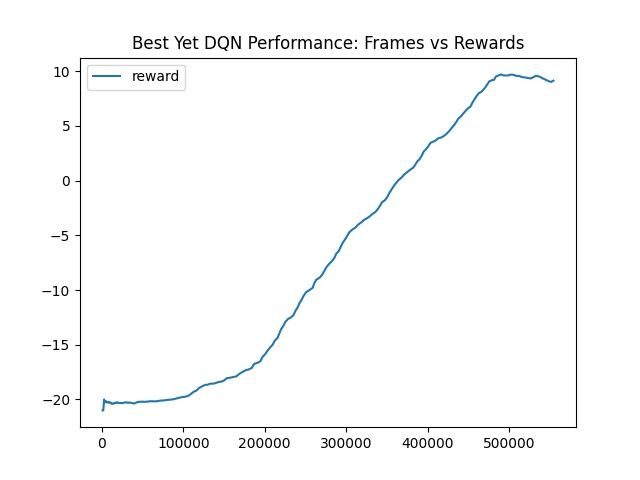
\includegraphics[width=\textwidth]{frame-reward.jpg}
                    \caption{A plot of the number of frames vs the average cumulative reward per game}
                \end{subfigure}
                \hfill
                \begin{subfigure}[b]{0.4\textwidth}
                    \centering
                    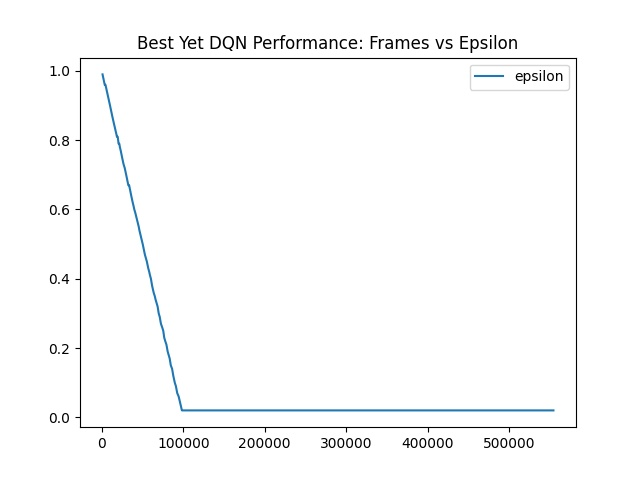
\includegraphics[width=\textwidth]{frame-epsilon.jpg}
                    \caption{A plot of the number of frames vs epsilon (from $\epsilon$-greedy approach)}
                \end{subfigure}
                \caption{Some metrics for the DQN}
            \end{figure}

        \section{Data Generation} 
            \par 500,000 frames of data are used in training. The frames are stacked one on top of the other, 4 at a time, thus 2 million frames must really be generated. In addition to the frames themselves, the action and reward must also be saved. We have simple extended the Replay Buffer from the DQN to get the frames. 50,000 frames (counting a stack of 4 as 1) were also generated for training.
        
        \section{Model Implementation}
            \par Create Autoencoder with action conditional representation added to the latent encoding. . We made a static auto encoder with three convolutional layers for encoding and decoding respectively and two linear layers before and after the transformation. To implement the model we used 2d convolution and linear layer implementation by Pytorch library. The input to the model were 1* 84 *84 grey scale images which were produced by the DQN model in previous step. As suggested in the paper all weights in the network were initialized according to (Glorot and Bengio, 2010). The images were pre-processed so that each pixel has range of [-1,1]. The layers which were a part of element wise multiplication that is the action processing layer, their weights were initialized in the range of [-1,1]. The action was fed in through the DQN model in the previous step and then passed through a fully connected layer for the transformation phase where it was integrated with the compressed latent representation of input frames.
            \begin{figure}[h!]
                \centering
                \begin{subfigure}[b]{\textwidth}
                    \centering
                    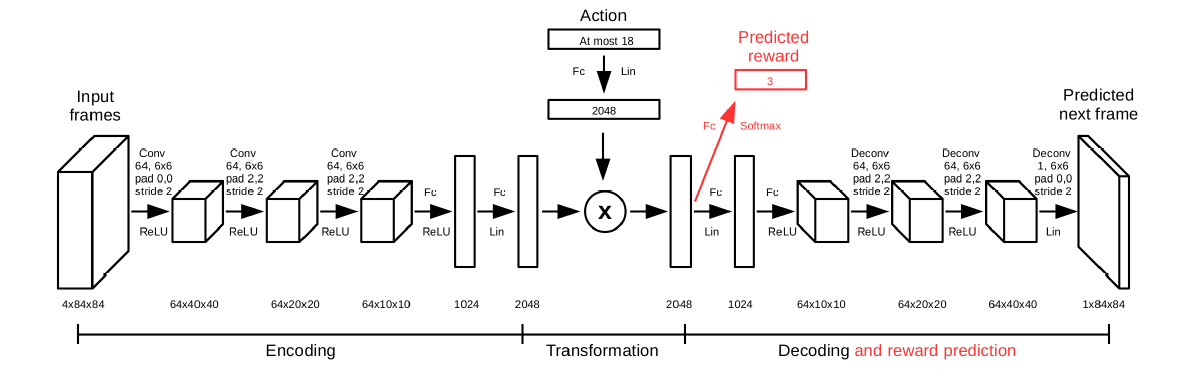
\includegraphics[width=\textwidth]{Model.jpg}
                    \caption{The architecture of the model.}
                \end{subfigure}
                \hfill
                \begin{subfigure}[b]{\textwidth}
                    \centering
                    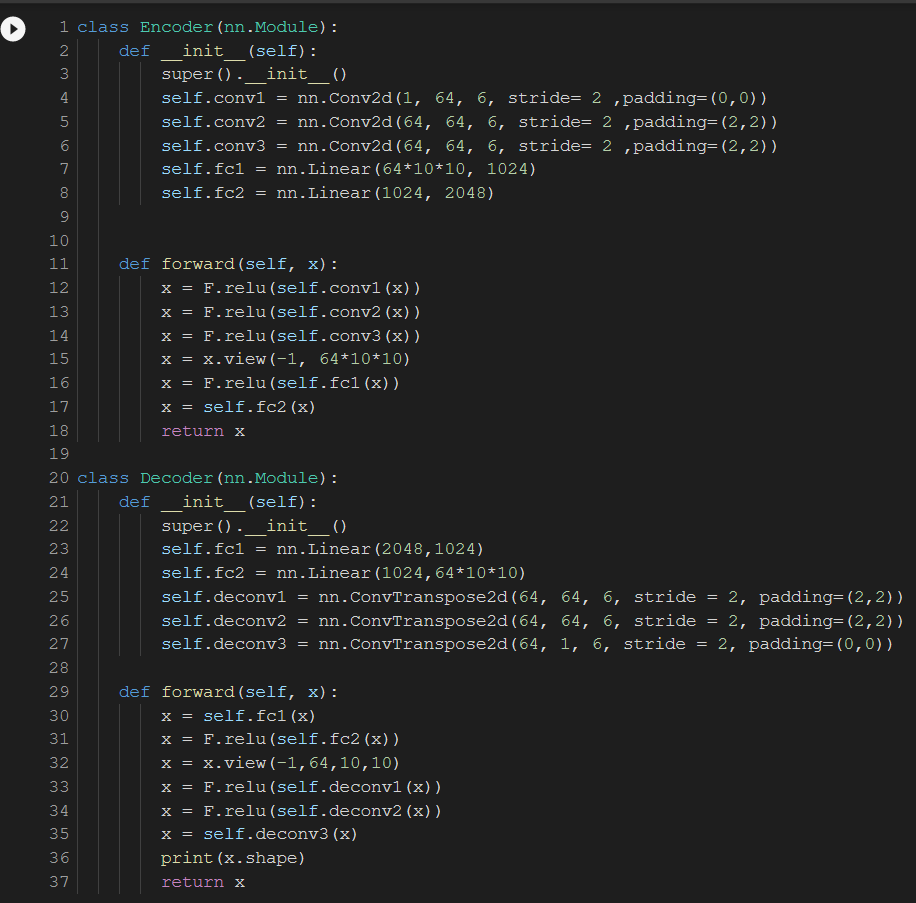
\includegraphics[width=\textwidth]{Encoder-Decoder.png}
                    \caption{The code for the encoder and decoder.}
                \end{subfigure}
            \end{figure}

        \section{Training} 
            \par Train the model by using Curriculum Learning through the new combined video frame prediction and cross-entropy reward prediction loss given in the paper. [Add citation] In curriculum learning the look ahead parameter is increased every 500,000 steps. This enables the model to slowly learn to predict farther and farther into the future. The Cost Function combines reward estimation and video frame prediction.
            \begin{figure}[h!]
                \centering
                \begin{subfigure}[b]{\textwidth}
                    \centering
                    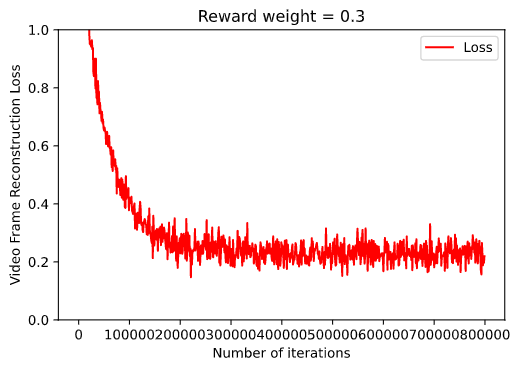
\includegraphics[width=\textwidth]{video-frame-reconstruction-loss.png}
                    \caption{The Video Frame Reconstruction Loss that we obtained. The graph is noisier, both since the reward weight is slightly higher and no smoothing has been done. Additionally, due to lack of access to powerful graphic cards, we were only able to plot the graph till 800k frames.}
                \end{subfigure}
                \hfill
                \begin{subfigure}[b]{\textwidth}
                    \centering
                    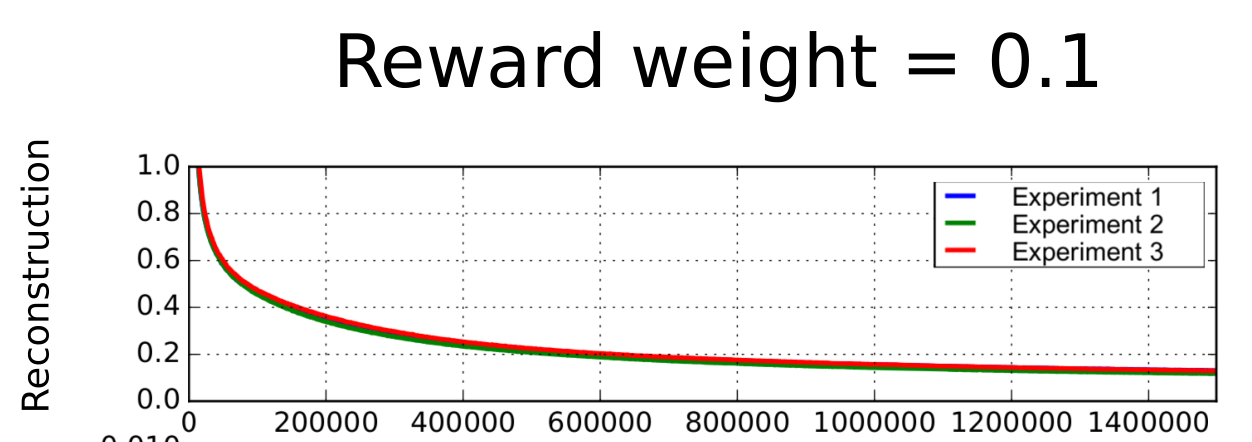
\includegraphics[width=\textwidth]{reconstruction-loss-in-paper.png}
                    \caption{The reconstruction loss from the paper. Exponential smoothing with a window size of 1000 has been done.}
                \end{subfigure}
                \caption[Reconstruction Loss comparison]{Reconstruction Loss comparison, between implementation and paper.}
            \end{figure}

        \section{Testing} 
            \par Testing involved seeing how far (in terms of look ahead steps) the model could accurately predict.
            \begin{figure}[h!]
                \centering
                \begin{subfigure}[b]{0.3\textwidth}
                    \centering
                    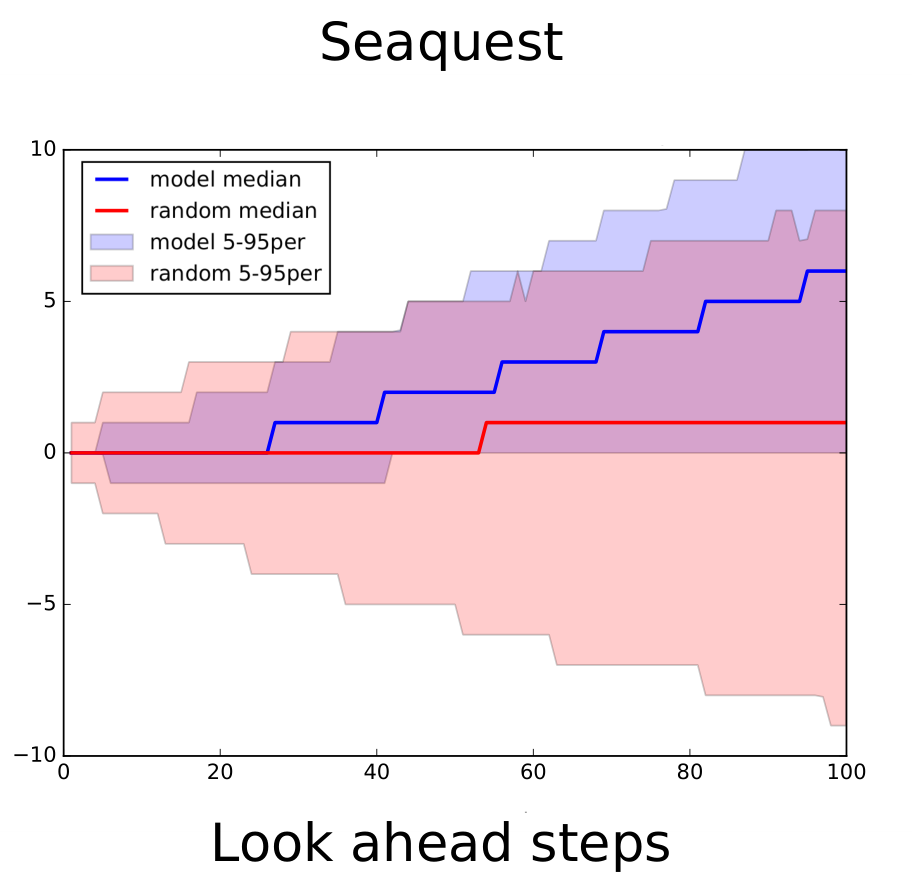
\includegraphics[width=\textwidth]{median-reward-seaquest.png}
                    \caption{Seaquest}
                \end{subfigure}
                \begin{subfigure}[b]{0.3\textwidth}
                    \centering
                    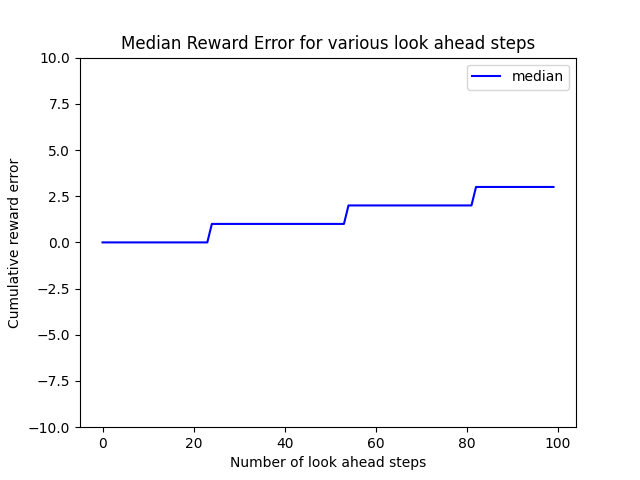
\includegraphics[width=1.2\textwidth]{median-reward-error.png}
                    \caption{Pong}
                \end{subfigure}
                \hfill
                \begin{subfigure}[b]{0.3\textwidth}
                    \centering
                    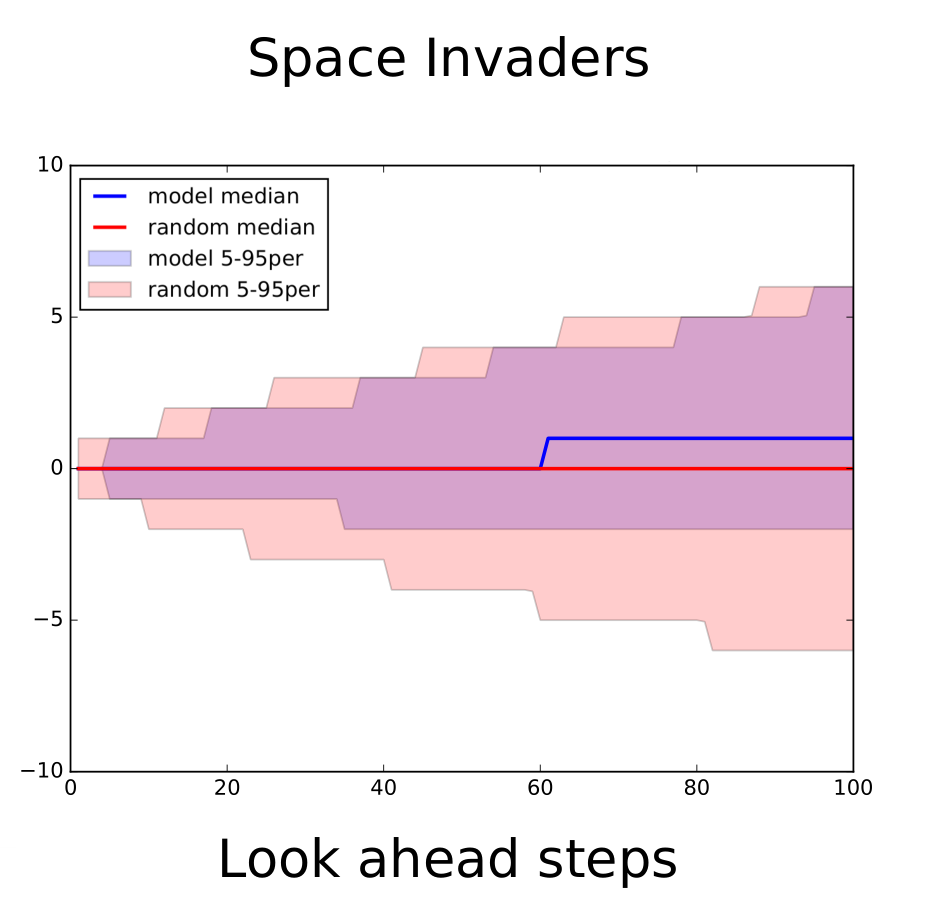
\includegraphics[width=\textwidth]{median-reward-space-invaders.png}
                    \caption{Space Invaders}
                \end{subfigure}
                \caption[Median cumulative reward error comparison]{Comparison of the median cumulative reward error for Seaquest, Space Invaders (from the paper) and Pong. As we can see, Space Invaders is much easier for the model than Seaquest. This is possibly because of the higher frequency of unpredictable, random events. Since even the opponent (controlled by the computer) in Pong is quite predictable, its mean reward error is more similar to Seaquest.}
            \end{figure}

    \chapter{Improvement Implementation and Results}
            \par The improvement that we were considering was to incorporate a Variational Autoencoder in-place of the regular Autoencoder. In a Variational Autoencoder instead of mapping an input to a fixed vector we map it onto a distribution. This introduces 2 new vectors: one for the mean and one for the standard deviation. And the problem of doing backpropagation through this is solved by re-parameterization, where we represent the sampled latent vector in terms of the mean and standard deviation. 

            \par During implementation stage we struggled a lot with re-parameterization and were ultimately unsuccessful in creating an error free implementation. The structure of the reward loss was such that it first decreased and then increased.
            \begin{figure}[h]
                \centering
                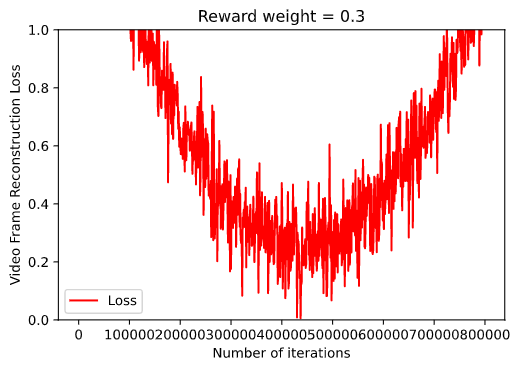
\includegraphics[width=\textwidth]{vae.png}
                \caption{Variational Autoencoder Video frame Reconstruction Loss}
            \end{figure}
    
    \chapter{Main Findings}
        \par We were successful in recreating the basic results of the paper. The look ahead values and the reward loss was comparable. 

        \par After training for over 7 hours and over 5,00,000 iterations the reward of the initial DQN model peaked at 10.23. We tried several implementations of it and changing the decay rate and update frequency we found the best decay rate and update frequency 100000 and 10k respectively. The other hyperparameters we are using are 0.00025 as learning rate,  0.99 discount factor and 32 as mini batch size.
    
    \chapter{Members and Their Contributions}
            \begin{enumerate}
                \item \textbf{Danish Mohammad} extracted the training images using the DQN model and made the reward structure for the baseline model, trained the main model on google colab.
                \item \textbf{Ashna Swaika} made the simple autoencoder model and worked with the variational auto encoder model
                \item \textbf{Aayush Jain} made the simple autoencoder and  worked with the variational autoencoder implementation and tried out several modifications
                \item \textbf{Rickston Pinto} Worked with the transformation phase and integrating the action vector with autoencoder phase. Also helped with variational autoencoder
            \end{enumerate}
\end{document}
